\label{sec:theory}
% Theoretical arguments in the literature closely related to your study
In this section we briefly relate the market for commercial air transport to network theory. We first present basic characteristics of air transport. We present the network theory most pertinent to our analysis including the measures we use to both characterize the network and expand the feature set for the predictive model. The last subsection describes how we build a prediction model.
%We draw on network theory to characterize how airports are connected to each other and analyze what role the individual airport plays in the network of airports. The ultimate aim of this analysis is to assess whether flight prices between airports depend on the role each airport plays in the network.\par
%We view airports as nodes in the network, with flights (or connections) representing links between airport. In connecting the network theory to the reality of the air transport market we use the terms interchangeably. Two airports are linked if there is at least one commercial flight between them in the time frame considered.

\subsection{Airline business models}
As is apparent in section \ref{sec:background}, the common view within academia is that large airlines specialize in either of two mayor business models with very distinct network characteristics. That is, legacy airlines lean towards managing a hub-and-spoke network while low cost carriers (LCC) lean towards offering point-to-point connections. \citep{daraban2012low,baker2013service,marti2015efficiency}.

\subsubsection{Point-to-point connections (T)}
Point-to-point connections are direct connections between two nodes. In aviation terminology it is routes connecting airports by direct flights as opposed to requiring transfers or layovers. The extreme being the fully-connected network in which every node is directly connected to each of the other nodes. While one can get anywhere in the network without wasting time and fuel by transferring in a hub, this also means that the required number of links, and thus carriers, grows exponentially with the number of nodes $N$ such that the number of links $L$ are \citep{bryan1999hub}:
\begin{equation}
  L=\frac{N\cdot(N-1)}{2}
  \label{eq:max_links}
\end{equation}
As noted by \citet{barabasi2016networks} this will also be the maximum number of links in any non-directed network. That is, a complete graph of just 7 nodes would have no less than 21 links as seen in the left panel of figure \ref{fig:different_networks} below.

\subsubsection{Hub-and-spoke network (M)}
The other extreme would be the single-hub or two-hub network where $N$ nodes would only need $N-1$ connections as the $N_s$ non-hub nodes, so called spokes, would only need to be connected to a hub in order to be indirectly connected to every other node in the network. \citet{o1987quadratic} presented a hub-and-spoke network as a simple single-assignment model such that non-hub nodes only have one link, namely the one connecting them to a hub.
\par
Given that all hubs are interlinked, drawing a few examples by hand will quickly reveal that the number of links $L_{HS}$ in a stylized hub-and-spoke network depends on the number of hubs $N_H$ and spokes $N_S$ in the following way
\begin{equation*}
  L_{HS}=\frac{N_H\cdot(N_H-1)}{2}+N_S,\ \ \ \ \ N_H>0
\end{equation*}
As seen in the middle panel of figure \ref{fig:different_networks} the two-hub network of 7 nodes only requires 6 links, however, the average shortest path length is $2$ as opposed to $1$ in the fully connected network (see paragraph \ref{par:shortest_path}).

\subsubsection{Focus cities (C)}
\label{subsec:focus_cities}
A third business model can be added, namely the concept that smaller regional airlines mainly serve the so-called spokes \citep{forbes2007role}. They usually serve as an integrated part of a hub-and-spoke network connecting the spokes to close-by hubs with smaller regional jets. However, regional airlines might also connect spokes to other spokes or even offering (infrequent) longer-range connections to other hubs, turning the spoke into a so called \textit{focus city} or tiny hub \citep{mammarella2014encyclopedia}.
\par
Likewise some airlines are combining the two structures such as the LCC \textit{Frontier Airlines} which first-and-foremost runs a hub in Denver. However, in 2012 they started experimenting with a new business model by expanding their service through offering long distance point-to-point flights to four popular West coast hubs via full-size jets from the small airport Colorado Springs (COS), just 90 miles (145 km) south of Denver International Airport.\footnote{\href{https://web.archive.org/web/20160526231749/http://gazette.com/springs-is-frontiers-new-front-in-battle-for-colorado-travelers/article/137275}{http://gazette.com/springs-is-frontiers-new-front-in-battle-for-colorado-travelers/article/137275}} This motivates us to choose COS as the airport for which we look into network changes over time in figure \ref{fig:map_COS}, section \ref{subsec:empirical_network_characteristics}.
\medskip\\
In the right panel of figure \ref{fig:different_networks} the spokes in the upper-right corner has been turned into a focus city, thus, cutting off one transfer in order to get to one of the airports in the lower half of the network. While this can be seen as deviance from the very strict definition of the stylized hub-and-spoke network \citep{o1987quadratic} we instead take on a looser approach in order to apply 'hub-and-spoke' as the best  overall characterisation whenever we observe a network similar to the one we see in the right panel of figure \ref{fig:different_networks}.
\begin{figure}[H]
  \centering
  \caption{Three different networks connecting 7 nodes}
    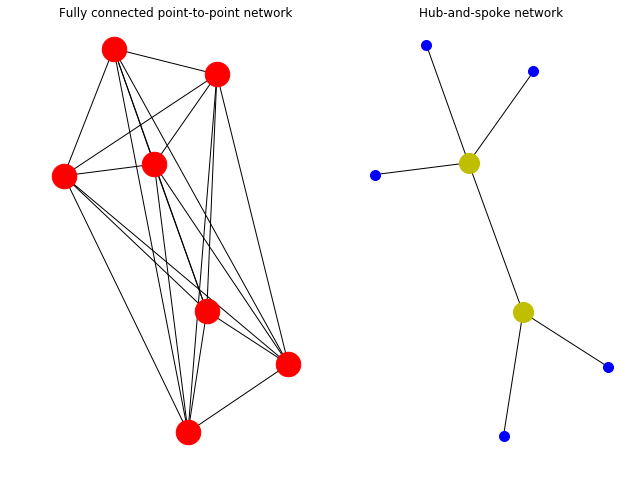
\includegraphics[width=\linewidth]{Exam/Figures/network_types}
    \vspace{-0.7cm}
  \label{fig:different_networks}
\end{figure}

\subsection{Network Theory}
\label{subsec:Network Theory}
We draw on network theory to characterize how airports are connected to each other and analyze what role the individual airport plays in the network of airports. %The ultimate aim of this analysis is to assess whether flight prices between airports depend on the role each airport plays in the network. \\

\subsubsection{Air transport as a scale-free network (T)}
A scale-free network is a network whose degree distribution follows a power law, i.e. $p_k \sim k^{-\gamma}$. One characteristic of the scale-free networks is the existence of 'hubs' - nodes that have a far higher degree than the average degree. Air transport is - quite literally - a textbook example of a scale-free network as seen in chapter 4 of \citet{barabasi2016networks}. In section \ref{sec:empirical} we will see that this is reflected in the degree distribution where most nodes have a low degree but some nodes (hubs) have a very high degree.
\par
Given this \textit{spoke-and-hub} nature of air transport, we expect the network to have some airports (hubs) that are connected to all or most other airports in its geographical vicinity, and well connected to similar hubs in other regions. This pattern may be repeating to some extent, insofar as there may be regional as well as national hubs.
\par
We further expect the network to be sparse, i.e. that the number of links is (far) lower than the number of possible links. This also reflects the hub-and-spoke nature of the network, in that small local airports are likely to have a low number of links, particularly relative to the possible number of links. However, we expect the network to be connected, in the sense that, given an appropriate time frame, there will always be a path from one airport any other (through some number of other airports).

\subsubsection{A Directed or Undirected Network (M)}
Although individual flights are clearly directed, going from one airport to the other, we will primarily view the network as undirected. The reason being, that connections between airports are typically undirected.
\par
As we will see in the data analysis, flights from airport $i$ to airport $j$, almost always implies flights from airport $j$ to airport $i$. We believe that this slight simplification to the network of airports is well suited for our analysis, that focuses exclusively on the effect on prices. An analysis of e.g. how delays propagate through the network, would require viewing links as directed and including time in a more intricate manner.

\subsubsection{Weighted Network and Temporal Considerations (C)}
We view the network as unweighted, that is, all links are considered to be equal. While this somewhat simplifies the analysis, we could have chosen to weight links e.g. by letting the number of flights between two airports determine the 'weight' of their common link.
\par
The considered time frame clearly matters for the characteristics of the network, since not all flights between airports take place every day or even every week. Considering a years worth of flights will produce far more links in the network than considering the flights that take place on a particular day. We choose to analyze the yearly network, to ensure that we also capture flights (links) that are seasonal in nature, e.g. flights that only happen in the summertime, or close to specific holidays.

\subsubsection{Selected Network Measures (T)}
In the course of the analysis, we draw upon a variety of measures to characterize the network. In the selection of measures, we look to \citet{chi2004structural}. The measures we have chosen to use are presented below. They are: Average degree, clustering coefficient, diameter, average shortest path length and betweenness centrality.

\paragraph{Average Degree}\mbox{} \\
The degree $k_i$ of node \textit{i} is the number of nodes with which node \textit{i} share a link. In our case the degree of an airport is the number of airports to which it has a flight connection. The average degree is then simply the average across nodes. Average degree is calculated as: 
\begin{align}
    \text{Average degree} = \frac{1}{N} \sum_{i = 1}^N k_i = \frac{2L}{N}
\end{align}

\paragraph{Clustering Coefficient} \mbox{} \\
The clustering coefficient for a given node \textit{i} is given as: 
\begin{align}
    C_i = \frac{2L_i}{k_i(k_i-1)}
    \intertext{Where $L_i$ denotes the number of links between node \textit{i}'s neighbors. The clustering coefficient of the network is then given by:}
    C = \frac{1}{N} \sum^N_{i=1} C_i
\end{align}
The clustering coefficient for a single node is equal to the fraction of possible links between node \textit{i}'s neighbors (nodes it is connected to) that are found in the network. A node whose neighbors are all connected to each other will have a clustering coefficient of 1. Conversely, if none of the nodes neighbors are connected, it will have a clustering coefficient of 0. Note, that for nodes with degree 1, the clustering coefficient is necessarily 0.

\paragraph{Average Shortest Path Length}\mbox{} \label{par:shortest_path} \\
The average shortest path length is defined as: 
\begin{align}
    a = \sum_{s,t \in V} \frac{d(s,t)}{N(N-1)}
\end{align}
Where $V$ is the set of nodes in the network, $d(i,j)$ is the length of the shortest path between nodes \textit{i} and \textit{j}, and $N$ is the number of nodes.

\paragraph{Diamater} \mbox{} \\
The diameter is the maximum shortest path length between any two nodes in the network. 

\paragraph{Betweenness Centrality}\mbox{} \\
Finally, we also calculate the betweenness centrality. For node \textit{i}, this is the fraction of shortest paths between all nodes in the network that pass through node \textit{i} \citep{brandes2008variants}.

\subsection{Prediction Model (M)}
\label{subsec: prediction model}
Based on the available data we want to assess whether network characteristics can improve a prediction model for flight prices. The simplest way of predicting a continuous variable is to use a linear regression model. We write our prediction model as
$$
y_i = w_0 + W X_i 
$$
where $y_i$ is the price of a given flight, $w_0$ is the bias/intercept, $X_i$ is a vector of features, and $W$ is a vector of corresponding weights. 
\medskip\\
To find the weights that makes the most accurate predictions we need to define a cost function. The standard cost function estimating a linear model is the \textbf{Mean Squared Error (MSE)}:
\begin{align}
\text{MSE}=\frac{1}{N} \sum_i^N (y_i - (w_0 + WX_i))^2
\end{align}
To address the problem of overfitting, we regularize the model using \textit{elastic net}, which combines L1 ("Lasso") and L2 ("Ridge") regularization. Each of these regularization methods work by adding a term to the cost function. In the case of Lasso, the cost function then becomes: 
\begin{align}
    J(w) = \sum^N_{i=1} (y_i-\hat{y}_i)^2 + \alpha \cdot \sum_{j=1}^p |w_j|
    \intertext{where $p$ is the number of features in the model. The hyper-parameter $\alpha$ then controls the strength of the regularization. In the case of Ridge regularization, the cost function becomes:}
     J(w) = \sum^N_{i=1} (y_i-\hat{y}_i)^2 + \alpha \cdot \sum_{j=1}^p w_j^2
\end{align}
Ridge regularization shrinks the weights in the model while Lasso tends to drive some coefficients to zero. Elastic net combines the two regularization methods, and adds an additional hyperparameter, the L1-ratio, that determines the relative importance of Ridge- and Lasso regularization. The model is numerically optimized using gradient descent.

\subsubsection{Model evaluation (C)}
In order to evaluate how our model performs on new data, we start by splitting the data into a training set and test set, keeping the latter untouched till the final model evaluation. The model is estimated using k-fold cross validated grid search. When estimating the model we are only using the training data. This allows us to get an unbiased estimate of the performance when we evaluate the model on  the test data.
\par
Estimating the model consists of two parts: one is to find the optimal weights in our prediction model - the other is to choose the optimal hyperparameters. The k-fold cross-validation randomly splits the training data into k folds, and then uses k-1 folds to train the model to optimize it before evaluating performance on the last fold. This procedure is then repeated k times, so that we obtain k models and the resulting score is an average of these k models. This k-fold cross-validation is done for each set of hyperparameter in the Cartasian product of the hyperparameters and the set of hyperparameters that performs the best are chosen. Finally, the model is evaluated on the test data.
